\documentclass[10pt,twocolumn,letterpaper]{article}

\usepackage[letterpaper,top=0.72in,bottom=0.78in,left=0.68in,right=0.68in,columnsep=0.24in]{geometry}
\usepackage{newtxtext}
\usepackage{microtype}
\usepackage{graphicx}
\usepackage{booktabs}
\usepackage{multirow}
\usepackage{array}
\usepackage{amsmath,mathtools}
\usepackage{newtxmath}
\usepackage{enumitem}
\usepackage[numbers,sort&compress]{natbib}
\usepackage{xcolor}
\usepackage[hidelinks]{hyperref}
\usepackage[font=small,labelfont=bf]{caption}
\usepackage{subcaption}
\usepackage{url}

\graphicspath{{../docs/figures/}}
\setlength{\parindent}{1em}
\setlength{\parskip}{0pt}
\setlength{\textfloatsep}{8pt plus 2pt minus 2pt}
\setlength{\floatsep}{7pt plus 2pt minus 2pt}
\setlength{\intextsep}{7pt plus 2pt minus 2pt}
\setlist{nosep,leftmargin=*}
\renewcommand{\arraystretch}{1.08}
\newcommand{\ie}{i.e.,\ }
\newcommand{\eg}{e.g.,\ }
\newcommand{\etal}{et al.}
\newcommand{\pp}{\,pp}
\newcommand{\method}{architecture-aware IMC-STE}
\newcommand{\E}{\mathbb{E}}
\newcommand{\R}{\mathbb{R}}

\title{\vspace{-0.48in}\Large\bfseries
Architecture-Aware Straight-Through Estimation\\
for Robust Analog In-Memory Computing\vspace{-0.10in}}
\author{Xin Su}
\date{}

\begin{document}
\maketitle
\vspace{-0.38in}

\begin{abstract}
Analog in-memory computing (IMC) can execute matrix--vector products with high
parallelism, but programming error, drift, asymmetric nonlinearity,
quantization, crosstalk, and read noise jointly make deployment operators both
stochastic and non-smooth.  We present an architecture-aware straight-through
estimation framework that exposes one noisy operator across linear, dense
convolution, grouped convolution, and depthwise convolution layers while using
controlled surrogate gradients for training.  The framework combines
saturation-aware backward estimators with a forward error decomposition that
separates stochastic read variation from systematic saturation bias.  This
decomposition motivates a clean-statistics activation preconditioner and
layer-type-aware repeated reads without reducing the noise assigned to any
individual operation.  Under a strict protocol in which every convolution and
linear layer uses the full challenge noise model, all six settings improve by
4.24--75.80 percentage points over direct noisy deployment, and four improve by
at least 29.21 points.  Five settings retain 86.60--94.78\% of clean accuracy.
On the most fragile case, TinyImageNet with EfficientNet-B0, direct
deployment obtains 0.50\% top-1 accuracy; preconditioned STE with depthwise and
pointwise repeated reads reaches $76.30\%\mathbin{\pm}0.25\%$ (95\% CI), versus
81.00\% clean.  A variance-guided 4--8-read policy reduces sensitive-layer
reads by 25.5\% and measured full-validation time by 23.0\% with no significant
accuracy change.  We also identify the limits of backward-only variance
scaling and report corrected shared-read semantics for memory-bounded
large-image convolution.
\end{abstract}

\section{Introduction}
\label{sec:introduction}

Analog IMC arrays reduce data movement by storing weights and performing
multiply--accumulate operations in the same physical substrate
\citep{gokmen2016acceleration,legallo2018mixed,shafiee2016isaac}.  Their analog
nature, however, introduces errors that do not resemble a single independent
Gaussian perturbation.  Programmed conductances vary, drift and retention alter
weights over time, nonlinear transfer functions saturate large partial sums,
and readout circuits add quantization, spatially correlated noise, and global
supply fluctuations.  Hardware-aware training can recover substantial
accuracy when the noise model is known \citep{joshi2020accurate}, but a general
training interface must also remain numerically useful when the simulated
forward contains random sampling and non-differentiable quantization.

Straight-through estimation (STE) replaces an unusable local derivative with a
surrogate during backpropagation \citep{bengio2013estimating}.  It is widely
used for binary and quantized networks
\citep{courbariaux2015binaryconnect,hubara2016binarized,yin2019understanding},
yet applying it to IMC raises two additional problems.  First, the forward error
has both random and systematic components; repeated reads reduce the former but
cannot remove saturation bias.  Second, layer topology matters.  A residual
network dominated by dense $3\!\times\!3$ convolutions and an EfficientNet
dominated by depthwise and pointwise operators can react very differently to
the same nominal nonidealities.

This work studies that interaction under the 2026 INNO IMC challenge
specification \citep{inno2026challenge}.  We deliberately use a strict
evaluation protocol: every convolution and linear layer receives the complete
noise configuration at scale 1.0.  Layer-wise noise reduction is evaluated
only as a diagnostic hardware-mapping bound and is excluded from the main
results.

Our contributions are fourfold:
\begin{itemize}
  \item We implement a common noisy/STE abstraction for linear, dense,
  grouped, and depthwise convolution, including memory-bounded convolution with
  physical read state shared across implementation chunks.
  \item We develop saturation-, variance-, and channel-aware surrogate
  gradients and derive a biased non-convex SGD bound that makes their intended
  bias--variance trade-off explicit.
  \item We show that systematic saturation, rather than read variance alone,
  dominates sensitive EfficientNet layers.  A statistics-driven activation
  preconditioner preserves the clean linear map while keeping every physical
  noise coefficient unchanged.
  \item We evaluate six classification model--dataset pairs, perform repeated
  noisy evaluation and controlled ablations, quantify training cost on an RTX
  4090, and report detection/segmentation extensions with explicit scope
  limitations.
\end{itemize}

\section{Related Work}
\label{sec:related}

\paragraph{Analog IMC simulation and robust training.}
Resistive cross-point arrays have been studied for both dense and convolutional
network training \citep{gokmen2016acceleration,gokmen2017convolutional} and for
mixed-precision computation \citep{legallo2018mixed}.  Hardware-aware noise
injection can preserve near-digital inference accuracy on phase-change memory
\citep{joshi2020accurate}.  AIHWKit provides configurable PyTorch simulation of
crossbar nonidealities \citep{rasch2021aihwkit}.  Noise-aware normalization
\citep{tsai2020noiseaware} and error suppression/compensation
\citep{eldebiky2022correctnet} address activation distribution shift and error
amplification.  Our focus is complementary: a generic surrogate-gradient
interface for a challenge-defined composite operator, with explicit treatment
of architecture-dependent saturation and read semantics.

\paragraph{Surrogate gradients.}
The STE copies or modifies an upstream derivative through a stochastic or
piecewise-constant operation \citep{bengio2013estimating}.  BinaryConnect and
binarized neural networks established its practical value
\citep{courbariaux2015binaryconnect,hubara2016binarized}; later analysis showed
that a suitable coarse gradient can align with a population gradient in
restricted quantized models \citep{yin2019understanding}.  Learned quantization
methods also scale surrogate gradients to stabilize trainable ranges
\citep{esser2020learned}.  In contrast to quantization-only work, our forward
includes stateful weight perturbations, asymmetric saturation, stochastic
readout, and correlated/global effects.  We therefore separate forward
conditioning from backward confidence scaling and test whether each supplies
independent empirical gain.

\section{Problem Formulation}
\label{sec:problem}

Let $X\in\R^{R\times I}$ and $W\in\R^{I\times O}$.  A noisy IMC operator
$\mathcal{N}_{\phi}(X,W;\xi)$ is parameterized by nonideality configuration
$\phi$ and random state $\xi$.  In compact form,
\begin{equation}
  \widetilde{Y}
  = \left[Q_b\!\left(h_{\alpha,\beta}
      ((X+\Delta X)(W+\Delta W))\right)
      + \Delta Y\right](1+\delta_s),
  \label{eq:noisy_operator}
\end{equation}
where $\Delta W$ combines programming, drift, retention, and temperature
terms; $\Delta X$ models input crosstalk; $\Delta Y$ combines independent and
spatially correlated output noise; and $\delta_s$ is a read-level supply
variation.  The asymmetric transfer function is
\begin{equation}
h_{\alpha,\beta}(z)=
\begin{cases}
\tanh(\alpha z)/\alpha, & z\geq 0,\\
\tanh((\alpha+\beta)z)/(\alpha+\beta), & z<0.
\end{cases}
\label{eq:saturation}
\end{equation}
The ADC operator $Q_b$ rounds to a signed $b$-bit grid and adds sub-step
quantization noise.  Appendix~\ref{app:noise} lists all coefficients.

For model parameters $\theta$, input--label pair $(x,y)$, and task loss
$\ell$, the robust objective is
\begin{equation}
  F(\theta)=\E_{(x,y)}\E_{\xi}
  \left[\ell(f_{\theta,\phi}(x;\xi),y)\right].
  \label{eq:objective}
\end{equation}
Direct differentiation through Eq.~\eqref{eq:noisy_operator} is ineffective at
the quantizer and can have excessive variance elsewhere.  We seek a surrogate
$\widehat{g}$ that remains informative while the forward pass exactly follows
the specified noisy operator.

\paragraph{Strict-noise protocol.}
The main experiments set a global noise multiplier to one for all nine
nonideality coefficients in every converted convolution and linear layer.  We
do not exempt first/last, depthwise, pointwise, or classifier layers.  Repeated
reads average independent applications of the same full-strength operator; they
do not attenuate the noise of an individual read.

\section{Architecture-Aware IMC-STE}
\label{sec:method}

\subsection{Generic Layer Conversion}

Model conversion recursively replaces $\texttt{Linear}$ and
$\texttt{Conv2d}$ modules while copying their parameters.  Convolution is
expressed as an unfolded matrix product.  Grouped convolution uses batched
grouped products,
\begin{equation}
Y_{r,g,o}=\sum_{k=1}^{I_g}X_{r,g,k}W_{g,k,o},
\label{eq:grouped}
\end{equation}
which keeps group weights isolated and makes depthwise convolution a special
case.  This gives all architectures the same forward noise implementation and
the same family of custom backward rules.

\subsection{Surrogate-Gradient Family}

For upstream gradient $G=\partial\ell/\partial\widetilde{Y}$, identity STE
uses the ideal local Jacobian:
\begin{equation}
  \widehat{\nabla_X\ell}=GW^\top,\qquad
  \widehat{\nabla_W\ell}=X^\top G.
  \label{eq:identity_ste}
\end{equation}
Saturation-aware STE multiplies $G$ by a softened derivative evaluated at the
ideal preactivation $Z=XW$:
\begin{equation}
  S(Z)=\gamma+(1-\gamma)
  \begin{cases}
  1-\tanh^2(\alpha Z),&Z\geq0,\\
  1-\tanh^2((\alpha+\beta)Z),&Z<0,
  \end{cases}
  \label{eq:saturation_scale}
\end{equation}
where $\gamma$ prevents complete gradient suppression.  Its adaptive variant
normalizes $S$ by the detached per-output mean and clips the result.

The variance-aware variant uses measured layer statistics.  If $r_{v,l}$ and
$r_{b,l}$ are stochastic- and bias-to-signal RMS ratios and $K_l$ reads are
averaged, layer confidence is
\begin{equation}
 c_l=\max\!\left(c_{\min},
 \left(1+\lambda_v r_{v,l}^2/K_l+lambda_b r_{b,l}^2\right)^{-1/2}\right).
 \label{eq:confidence}
\end{equation}
An optional channel vector $d_l$ further rescales $G$.  Ordinary, depthwise,
pointwise, and linear modules can carry separate profiles.  This design encodes
the fact that averaging reduces random variance approximately as $1/K_l$, but
does not reduce systematic bias.  Section~\ref{sec:ablation} shows that this
backward-only correction stabilizes gradients but is not the source of our
largest accuracy improvement.

\subsection{Statistics-Driven Activation Preconditioning}
\label{sec:preconditioning}

For each layer $l$, we collect the 99th percentile $q_l$ of the absolute clean
MAC output and define
\begin{equation}
  a_l=\operatorname{clip}(\tau/q_l,a_{\min},1),\qquad
  \widetilde{Y}_l=\frac{1}{a_l}\mathcal{N}_{\phi}(a_lX_l,W_l;\xi).
  \label{eq:precondition}
\end{equation}
We use $\tau=4$ and $a_{\min}=0.1$ for depthwise and pointwise layers.  In the
clean linear limit, $a_l^{-1}(a_lX_lW_l)=X_lW_l$, so the intended operator is
unchanged.  Unlike shrinking $W_l$ and amplifying the output, input scaling
does not amplify the first-order programming perturbation $X_l\Delta W_l$.
It does amplify additive output noise by $1/a_l$, which motivates the read
allocation below.  Statistics are frozen from the original clean checkpoint;
re-estimating them after noisy fine-tuning was empirically harmful.

We also evaluate bounded learned scales,
\begin{equation}
\begin{aligned}
 a_l&=a_{\min}+(a_{\max}-a_{\min})\sigma(\vartheta_l),\\
 R_a&=\frac{1}{L_a}\sum_l(\log a_l-\log a_l^{(0)})^2,
\end{aligned}
 \label{eq:learned_scale}
\end{equation}
initialized by Eq.~\eqref{eq:precondition}.  The constraint is essential: an
unconstrained scale sweep drifts out of the validated linear range.

\subsection{Read-Aware Training and Inference}

Exact $K_l$-read inference returns
\begin{equation}
  \overline{Y}_l=\frac{1}{K_l}\sum_{k=1}^{K_l}
  \mathcal{N}_{\phi}(X_l,W_l;\xi_{l,k}).
  \label{eq:reads}
\end{equation}
For EfficientNet-B0, training uses four reads on depthwise/pointwise layers and
evaluation uses eight.  To compensate for output-noise amplification in
Eq.~\eqref{eq:precondition}, an adaptive policy assigns
\begin{equation}
  K_l=\operatorname{clip}(\lceil K_0/a_l^2\rceil,K_0,K_{\max}).
  \label{eq:read_budget}
\end{equation}
We further implement a training-only moment-matched approximation that scales
zero-mean random terms by $1/\sqrt{K_l}$ while retaining nonlinearity and ADC
parameters.  Final evaluation always uses exact reads.

\subsection{Shared State for Chunked Convolution}
\label{sec:shared_read}

Large images make full unfold tensors prohibitively large.  We therefore chunk
the output rows, but sample weight-side programming, drift, retention,
temperature, and global supply state once per physical read and reuse it across
all spatial chunks and MAC tiles.  Input crosstalk and output read noise remain
location-specific.  Earlier per-chunk resampling introduced unintended spatial
averaging, so chunk size changed not only memory but also the physical model.
The shared-read state removes that confound while reducing the unfold workspace
from $\mathcal{O}(NH_oW_oC_ik_hk_w)$ to
$\mathcal{O}(Nh_cW_oC_ik_hk_w)$ for $h_c$ output rows per chunk.

\section{Optimization Analysis}
\label{sec:theory}

Let $\widehat g_t$ denote the STE gradient and write its conditional bias and
variance as
\begin{equation}
 \E_t[\widehat g_t]=\nabla F(\theta_t)+b_t,\qquad
 \E_t\|\widehat g_t-\E_t\widehat g_t\|^2\leq\sigma_g^2.
 \label{eq:bias_variance}
\end{equation}
The mean-squared estimation error is the sum of $\|b_t\|^2$ and the conditional
variance.  The online channel profile is a diagonal matrix $D_t$ with entries
in $[d_{\min},1]$, hence
\begin{equation}
 d_{\min}\|g\|_2\leq\|D_tg\|_2\leq\|g\|_2.
 \label{eq:bounded_scale}
\end{equation}
It cannot amplify high-variance channels, while the floor prevents complete
gradient loss.

\paragraph{Proposition 1.}
Assume $F$ is $L$-smooth and lower bounded by $F_*$,
$\|b_t\|\leq B$, and Eq.~\eqref{eq:bias_variance} holds.  For
$\theta_{t+1}=\theta_t-\eta\widehat g_t$ with
$0<\eta\leq1/(4L)$,
\begin{align}
\frac{1}{T}\sum_{t=0}^{T-1}\E\|\nabla F(\theta_t)\|^2
&\leq \frac{2(F(\theta_0)-F_*)}{\eta T}
 +2(1+L\eta)B^2+L\eta\sigma_g^2.
\label{eq:convergence}
\end{align}
The proof follows the standard smoothness descent argument
\citep{bottou2018optimization} and is given in Appendix~\ref{app:proof}.  For an
unbiased estimator and $\eta=\mathcal{O}(T^{-1/2})$, the average stationarity
measure has the usual $\mathcal{O}(T^{-1/2})$ behavior.  Biased STE converges
only to a neighborhood controlled by $B^2$.  This result motivates reducing
systematic saturation bias and random read variance separately; it does not
guarantee final classification accuracy, and the online profile's dependence on
the current batch requires additional assumptions for a sharper adaptive proof.

All clean, noisy, and single-read STE matrix products have leading arithmetic
cost $\Theta(RIO)$.  Exact $K$ reads cost $\Theta(KRIO)$.  Online paired
profiling adds one clean forward to the noisy forward/backward but does not
change the asymptotic order.  Persistent profile storage is only
$\mathcal{O}(C_{out})$ per layer and is disabled at deployment.

\section{Experiments}
\label{sec:experiments}

\subsection{Setup}

We evaluate ResNet18 \citep{he2016resnet} and EfficientNet-B0
\citep{tan2019efficientnet} on CIFAR-10/100 \citep{krizhevsky2009cifar} and
TinyImageNet \citep{le2015tinyimagenet}, an ImageNet-like 200-class subset
derived from the ImageNet hierarchy \citep{deng2009imagenet}.  TinyImageNet
uses 224-pixel inputs and ImageNet initialization.  CIFAR clean models are
trained for 120 epochs with SGD, cosine decay, AutoAugment, and label smoothing;
noisy fine-tuning starts from the corresponding clean checkpoint, uses gradient
clipping at 1.0, and selects a checkpoint using noisy validation.  TinyImageNet
protocols are detailed in Appendix~\ref{app:protocols}.

We compare (i) clean digital evaluation, (ii) direct noisy deployment of the
clean checkpoint, (iii) standard noisy training through the native simulated
graph, and (iv) identity, saturation-aware, and adaptive saturation-aware STE.
All reported main noisy results use the strict protocol in
Section~\ref{sec:problem}.  CIFAR results are means over five independent noisy
evaluations of a fixed trained checkpoint.  TinyImageNet ResNet18 and direct
EfficientNet results use three noisy evaluations; the final preconditioned
EfficientNet result uses five.  Thus these intervals measure deployment noise,
not full retraining uncertainty.  We report normal-approximation 95\% confidence
intervals and use paired $t$-tests when the same noise seeds are available;
Welch tests are used for unpaired comparisons \citep{welch1947ttest}.

\subsection{Strict Uniform-Noise Results}
\label{sec:main_results}

Table~\ref{tab:main_results} reports the clean, direct noisy, and best strict STE
result for each required classification pair.  STE recovers more than
$29\pp$ on both CIFAR-10 architectures and $33.84\pp$ on CIFAR-100 with
EfficientNet-B0.  CIFAR-100 with ResNet18 and TinyImageNet with ResNet18 are
harder relative cases: their direct noisy checkpoints are already less damaged,
and the best recovery is $6.98\pp$ and $4.24\pp$, respectively.

\begin{table*}[t]
\centering
\caption{Strict uniform-noise classification.  Noisy entries are repeated-evaluation means; $\pm$ denotes 95\% CI.  Recovery is best STE minus direct noisy.  No layer has reduced noise.}
\label{tab:main_results}
\scriptsize
\setlength{\tabcolsep}{4.2pt}
\begin{tabular}{lrrrrrl}
\toprule
Dataset / architecture & Clean & Direct noisy & Best strict & Recovery & Retained & Best strict protocol \\
\midrule
CIFAR-10 / ResNet18
  & 95.62 & $61.42\pm1.30$ & $\mathbf{90.63\pm0.19}$ & +29.21 & 94.78 & identity STE \\
CIFAR-10 / EfficientNet-B0
  & 91.13 & $38.93\pm0.60$ & $\mathbf{86.12\pm0.17}$ & +47.19 & 94.50 & saturation-aware STE \\
CIFAR-100 / ResNet18
  & 78.32 & $62.98\pm0.52$ & $\mathbf{69.96\pm0.33}$ & +6.98 & 89.33 & adaptive saturation STE \\
CIFAR-100 / EfficientNet-B0
  & 71.14 & $27.76\pm0.50$ & $\mathbf{61.60\pm0.32}$ & +33.84 & 86.60 & identity STE \\
TinyImageNet / ResNet18-224
  & 71.60 & $53.83\pm0.26$ & $\mathbf{58.07\pm0.53}$ & +4.24 & 81.10 & saturation-aware STE \\
TinyImageNet / EfficientNet-B0-224
  & 81.00 & $0.50\pm0.06$ & $\mathbf{76.30\pm0.25}$ & +75.80 & 94.20 & preconditioned STE + p/d read 8 \\
\bottomrule
\end{tabular}
\end{table*}

\begin{figure*}[t]
  \centering
  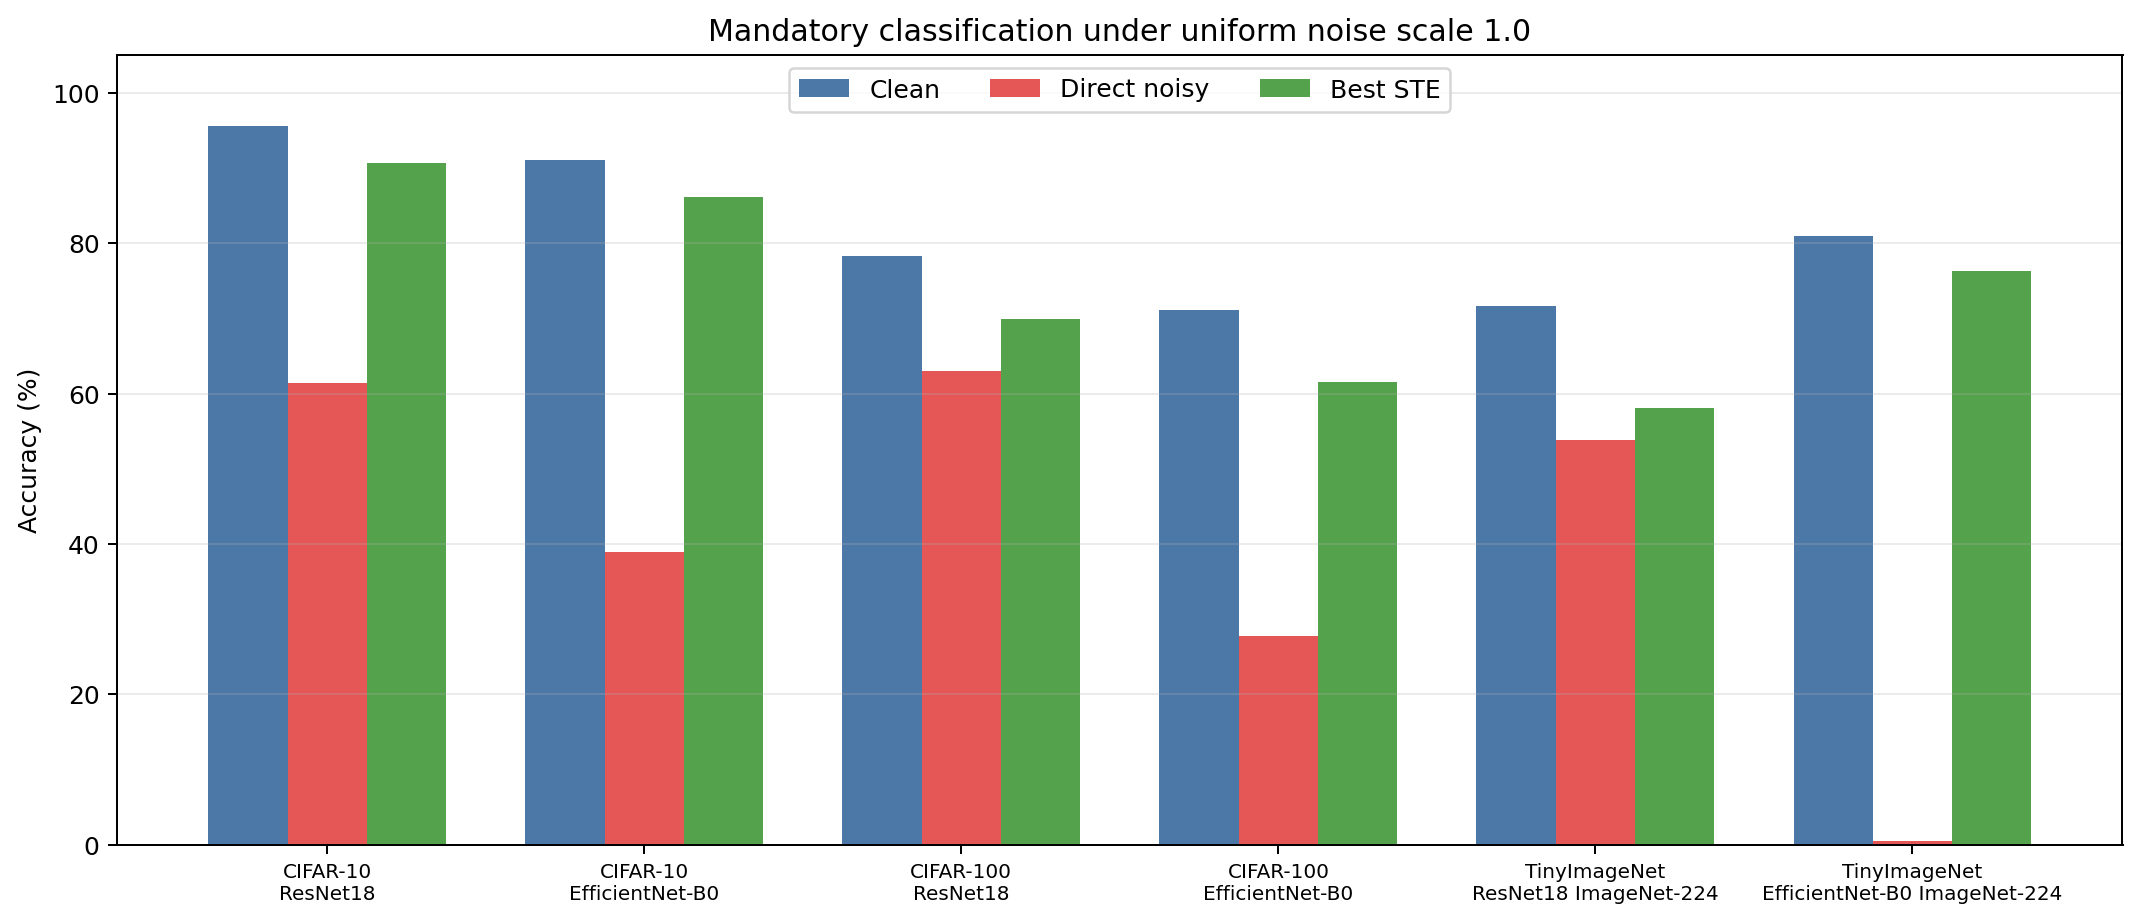
\includegraphics[width=0.96\textwidth]{submission_key_results.png}
  \caption{Clean, direct noisy, and best strict STE accuracy for all six
  classification pairs.  EfficientNet-B0 on TinyImageNet is the clearest
  architecture-dependent failure: the clean checkpoint is nearly random under
  direct deployment, while the proposed preconditioning/read-aware pipeline
  restores most clean accuracy.}
  \label{fig:key_results}
\end{figure*}

Table~\ref{tab:five_modes} isolates the effect of the backward estimator on the
four CIFAR settings.  Native noisy training improves over direct deployment,
but identity STE adds a further $6.71$--$15.96\pp$.  Saturation-aware scaling is
most useful for CIFAR-10 EfficientNet-B0, while identity STE is marginally best
on two settings.  This variability argues for exposing a strategy family rather
than assuming that a more elaborate surrogate is universally superior.

\begin{table}[t]
\centering
\caption{Five-mode CIFAR comparison under the same strict noisy evaluation
(top-1, \%).  ``Native'' differentiates the simulated graph directly.}
\label{tab:five_modes}
\scriptsize
\setlength{\tabcolsep}{3.1pt}
\begin{tabular}{lrrrrr}
\toprule
Task & Direct & Native & STE & Sat. & Adapt. \\
\midrule
C10 / R18  & 61.42 & 82.37 & \textbf{90.63} & 90.51 & 90.52 \\
C10 / Eff. & 38.93 & 68.44 & 84.40 & \textbf{86.12} & 86.03 \\
C100 / R18 & 62.98 & 63.20 & 69.91 & 69.88 & \textbf{69.96} \\
C100 / Eff.& 27.76 & 48.92 & \textbf{61.60} & 61.49 & 61.36 \\
\bottomrule
\end{tabular}
\end{table}

\subsection{EfficientNet Requires Forward Conditioning}
\label{sec:efficientnet}

TinyImageNet EfficientNet-B0 exposes a failure that backward tuning alone does
not solve.  Plain uniform-noise STE fine-tuning reaches 25.24\%; averaging eight
reads at all layers reaches 41.58\%, and restricting read-aware training and
evaluation to pointwise/depthwise (P/D) layers reaches 43.78\%.  Activation
preconditioning then raises the five-seed full-validation mean to 76.30\%, a
$32.52\pp$ improvement over the best read-only route.

\begin{table}[t]
\centering
\caption{TinyImageNet EfficientNet-B0 progression under strict per-read noise.}
\label{tab:tiny_progression}
\scriptsize
\setlength{\tabcolsep}{3.5pt}
\begin{tabular}{lr}
\toprule
Protocol & Top-1 (\%) \\
\midrule
Clean digital & 81.00 \\
Direct noisy, one read & $0.50\pm0.06$ \\
Uniform STE fine-tune, one read & $25.24\pm0.32$ \\
Uniform STE, all-layer read 8 & 41.58 \\
Read-adapted STE, all-layer read 8 & 42.61 \\
P/D read-aware STE, P/D read 8 & 43.78 \\
Preconditioned STE, P/D read 8 & $\mathbf{76.30\pm0.25}$ \\
Bounded learned scale, P/D read 8 & $76.37\pm0.14$ \\
Adaptive 4--8 reads & $76.20\pm0.05$ \\
\bottomrule
\end{tabular}
\end{table}

To identify the cause, we run one clean and four independent noisy forwards and
decompose mean squared error into total, stochastic, and residual systematic
components.  For depthwise layers, total/stochastic/systematic RMS-to-signal
ratios are 0.832/0.142/0.818; for pointwise layers they are
0.883/0.236/0.838.  Thus most error energy is systematic.  The large jump from
43.78\% to 76.30\% is consistent with moving pre-BN MAC values away from the
asymmetric saturation regime, while repeated reads address the smaller random
component.

\begin{figure*}[t]
  \centering
  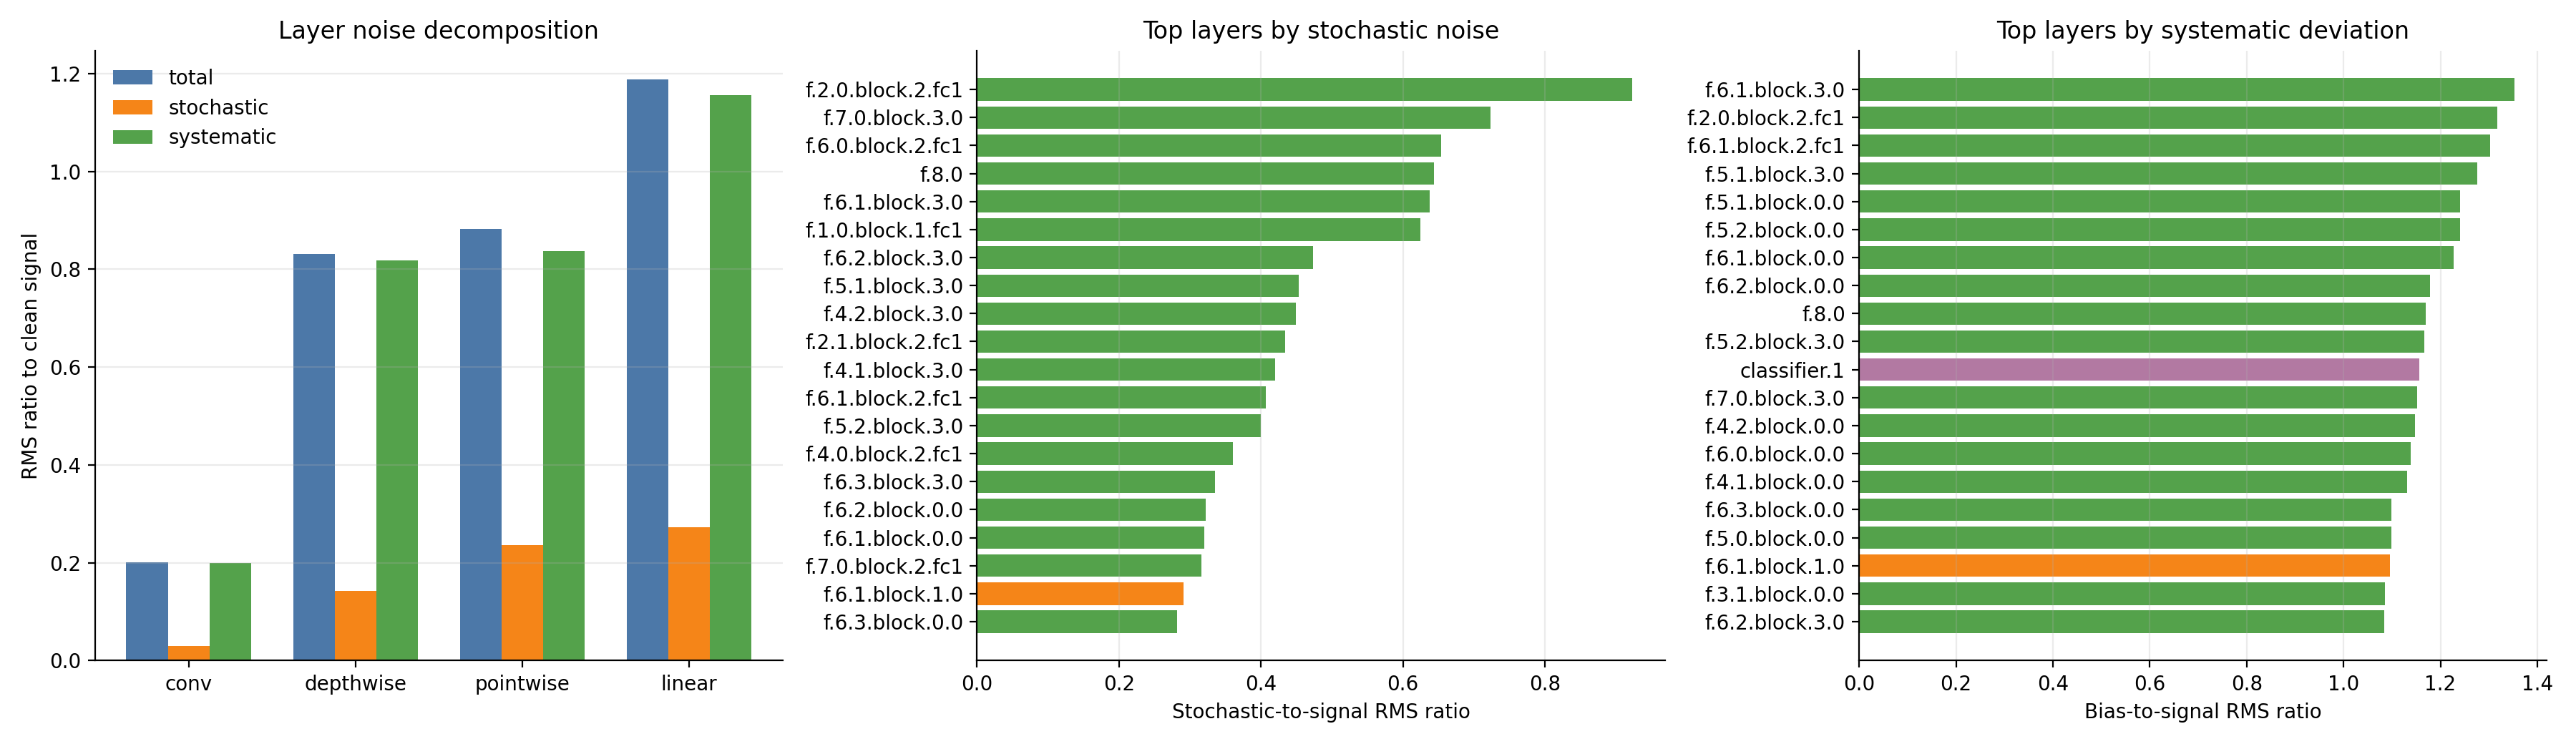
\includegraphics[width=0.99\textwidth]{tinyimagenet_efficientnet_b0_clean_layer_noise_decomposition_seed1.png}
  \caption{Layer error decomposition for the clean TinyImageNet
  EfficientNet-B0 checkpoint.  Left: type averages.  Center/right: layers with
  the largest stochastic and systematic components.  Systematic deviation
  dominates depthwise and pointwise layers, motivating forward preconditioning
  rather than backward variance scaling alone.}
  \label{fig:decomposition}
\end{figure*}

\section{Ablations and Efficiency}
\label{sec:ablation}

\subsection{Estimator and Scale Ablations}

On a matched 20-batch TinyImageNet comparison, backward-only variance/bias
confidence obtains 41.95\%, below the 42.27\% read-aware control.  With forward
preconditioning, identity and variance-aware STE both obtain 74.45\%, while the
combined variance/saturation variant obtains 74.30\%.  The principal gain is
therefore the forward transformation in Eq.~\eqref{eq:precondition}, not a more
complex backward rule.  This negative result is important: the framework can
express profile-aware gradients, but the data do not support claiming that they
outperform identity STE in the main classification setting.

Bounded learned scales move the three-seed paired mean from 76.28\% to 76.37\%,
an average $+0.09\pp$ with $p=0.247$.  The effect is not significant.  The
adaptive read policy assigns 477 total reads across 80 sensitive layers versus
640 for uniform eight-read inference, a 25.47\% reduction.  Its mean accuracy
is $0.073\pp$ lower with paired $p=0.568$, also not significant.  The same-seed
full-validation runtime falls from 300.21 to 231.25 seconds (22.97\%).

\begin{figure*}[t]
  \centering
  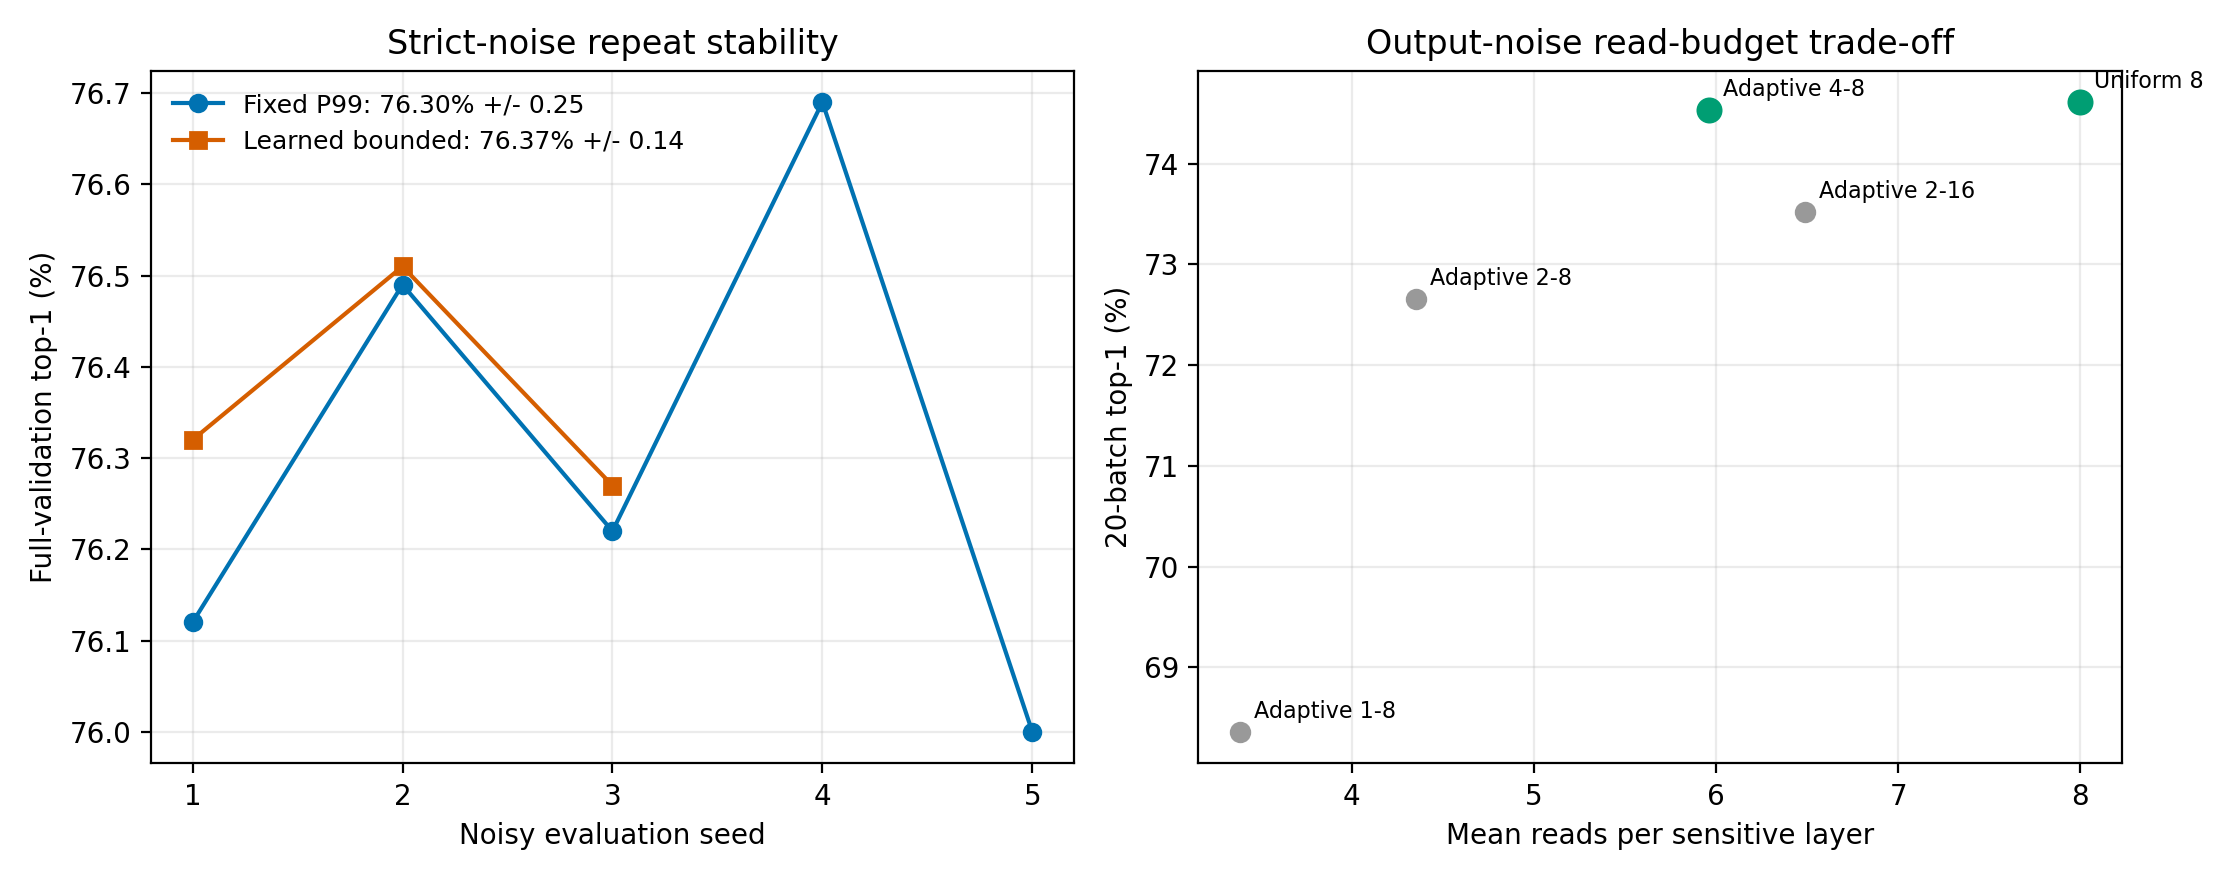
\includegraphics[width=0.94\textwidth]{tinyimagenet_efficientnet_b0_adaptive_scale_and_read_budget.png}
  \caption{Left: repeated full-validation accuracy for fixed P99 and bounded
  learned activation scales.  Learned-scale points are available for the first
  three matched seeds.  Right: accuracy versus mean sensitive-layer reads for
  several allocation policies.  Adaptive 4--8 reads preserve the uniform-eight
  operating point with lower logical read cost.}
  \label{fig:read_budget}
\end{figure*}

The training-only moment-matched approximation reduces a two-batch exact
eight-read benchmark from 48.59 to 1.00 seconds per batch (48.7$\times$), but
joint fine-tuning with this approximation does not improve final accuracy.
Accordingly, we use it only for low-cost training and retain exact reads for all formal
evaluations.

\subsection{Measured Training Cost}

We benchmark a CIFAR-stem ResNet18 on an RTX 4090 with PyTorch 2.6.0 and CUDA
12.6, batch size 8, ten warm-up steps, and fifty measured full training steps.
Each step includes forward, cross-entropy, backward, and SGD update.  Online
profiling includes its paired clean/noisy forwards.

\begin{table}[t]
\centering
\caption{RTX 4090 training-step microbenchmark.  Peak memory is incremental
allocated memory above the resident model baseline.}
\label{tab:efficiency}
\scriptsize
\setlength{\tabcolsep}{3.6pt}
\begin{tabular}{lrrr}
\toprule
Path & Step (ms) & Images/s & Peak MiB \\
\midrule
Clean & 4.87 & 1643.94 & 35.50 \\
Identity STE & 25.71 & 311.12 & 278.35 \\
Online profile STE & 47.96 & 166.80 & 296.45 \\
\bottomrule
\end{tabular}
\end{table}

Identity STE costs 5.28$\times$ clean in this software simulator.  Online
profiling costs 1.87$\times$ identity STE and adds 18.10 MiB incremental peak
memory, mainly because of the extra clean forward.  Profiling is training-only;
its buffers are non-persistent and incur no deployment inference cost.  These
numbers characterize this implementation, not analog hardware latency or
energy.

\section{Large-Image Cross-Domain Stress Test}
\label{sec:optional}

We connect the same internal noisy layers to Faster R-CNN
\citep{ren2015fasterrcnn} and DeepLabV3 \citep{chen2017deeplab} on PASCAL VOC
\citep{everingham2010voc}.  The purpose is to validate grouped conversion,
memory-bounded unfold, shared-read state, and task-head diagnostics.  These are
not the challenge's official COCO/Cityscapes optional benchmarks and must not be
interpreted as completing that optional track.

\begin{table}[t]
\centering
\caption{Corrected shared-read full-validation stress test.  STE uses one full
fine-tuning epoch and strict uniform noise.}
\label{tab:optional}
\scriptsize
\setlength{\tabcolsep}{4pt}
\begin{tabular}{lrrrr}
\toprule
Task / metric & Clean & Direct & STE & Recovery \\
\midrule
VOC07 Faster R-CNN / mAP50 & 72.59 & 28.72 & 37.53 & +8.81 \\
VOC12 DeepLabV3 / mIoU & 71.31 & 4.03 & 6.46 & +2.43 \\
\bottomrule
\end{tabular}
\end{table}

The low absolute results are diagnostic, not hidden successes.  Head-level
residual-to-signal ratios exceed one for detection ROI and segmentation
classifier modules.  A combination of online channel profiling,
pixel-logit consistency, and range control improves a matched segmentation
evaluation by $0.245\pp$ over three training seeds ($p=0.0086$, all seeds positive)
and preserves $+0.260\pp$ after one full epoch, but its 6.21\% absolute mIoU
does not exceed the 6.46\% formal run.  Detection profile and proposal-aligned
ROI variants remain seed-unstable.  We therefore retain the mechanism evidence
without promoting these candidates to main results.

\section{Limitations}
\label{sec:limitations}

First, the noise model is a software realization of the organizer-provided
operator, not a calibration to a specific fabricated array.  Accuracy cannot be
compared directly with silicon measurements under different devices, mappings,
or digital periphery.  Second, most classification confidence intervals vary
the noisy evaluation seed for one trained checkpoint; broader training-seed
replication remains desirable.  Third, TinyImageNet is an approved practical
ImageNet-like task but is not ImageNet-1K.  Fourth, multi-read inference trades
latency and energy for variance reduction; we measure simulator runtime and
logical reads, not hardware energy.  Fifth, the VOC experiments validate the
large-image mechanism but do not satisfy the official COCO/Cityscapes optional
protocol, and their absolute noisy accuracy remains low.  Finally,
Eq.~\eqref{eq:convergence} is a generic biased-gradient bound under smoothness
and bounded-moment assumptions, not a guarantee for arbitrary deep networks.

\section{Conclusion}

Complex IMC nonidealities require more than injecting scalar Gaussian noise.
The proposed framework keeps the full noisy forward while providing generic
surrogate gradients across dense, grouped, and depthwise operators.  Across six
strict classification settings, it recovers substantial deployment accuracy;
on TinyImageNet EfficientNet-B0 it restores a nearly random 0.50\% direct result
to $76.30\%\mathbin{\pm}0.25\%$, retaining 94.20\% of clean accuracy.  Layer
decomposition shows why: sensitive mobile convolutions are dominated by
systematic saturation bias, so statistics-driven forward preconditioning is
more effective than backward variance scaling alone.  Read-aware training then
addresses the remaining stochastic component, and an adaptive policy removes a
quarter of sensitive-layer reads without a significant accuracy change.  The
same implementation also exposes a crucial systems lesson for large images:
memory chunking must not silently resample physical weight state.  Together,
these results support architecture-aware forward conditioning, explicit read
semantics, and honest uncertainty reporting as central ingredients of robust
IMC training.

\bibliographystyle{unsrtnat}
\bibliography{references}

\clearpage
\appendix

\section{Noise Configuration}
\label{app:noise}

Table~\ref{tab:noise_config} lists the full-strength configuration used in all
strict experiments.  The global noise multiplier scales every floating-point
nonideality coefficient together and equals one in the main results.  It does
not alter the eight-bit ADC setting.

\begin{table}[h]
\centering
\caption{Strict noise parameters.}
\label{tab:noise_config}
\scriptsize
\begin{tabular}{lr@{\hspace{10pt}}lr}
\toprule
Parameter & Value & Parameter & Value \\
\midrule
Programming std. & 0.010 & Output std. & 0.010 \\
Drift factor & 0.005 & Crosstalk factor & 0.002 \\
Nonlinear $\alpha$ & 0.100 & Temperature factor & 0.001 \\
Asymmetry $\beta$ & 0.050 & Retention loss & 0.001 \\
Supply std. & 0.010 & ADC bits & 8 \\
\bottomrule
\end{tabular}
\end{table}

Programming noise is additive.  Drift is proportional to $|W|$, retention is
proportional to $W$, and temperature noise is proportional to $\sqrt{|W|}$.
Input crosstalk scales with each input row's vector norm.  Output noise contains
an independent component and a $3\times3$ spatially averaged component with
0.3 relative amplitude.  Supply variation is scalar within a physical read.

\section{Protocol Details}
\label{app:protocols}

\paragraph{CIFAR.}
Clean pretraining uses 120 full epochs.  The formal five-mode comparison uses a
two-stage clean-to-noisy procedure, learning rate 0.001 for the final 20-epoch
sweep, and gradient clipping at 1.0.  Earlier 40-epoch calibration runs are
retained for saturation-aware CIFAR-10 checkpoints when they provide the best
repeated noisy mean.  Comparisons within each task use the same strict noisy
evaluation configuration and full test set.

\paragraph{TinyImageNet ResNet18.}
The 224-input model uses ImageNet initialization.  The best strict result uses
saturation-aware STE at learning rate $5\times10^{-4}$ for ten epochs with 300
training batches per epoch.  Full validation contains 10,000 samples.

\paragraph{TinyImageNet EfficientNet-B0.}
The preconditioned route starts from the 81.00\% clean checkpoint.  Stage one
uses identity STE, four depthwise/pointwise reads, 50 batches, and learning rate
$5\times10^{-4}$.  Stage two uses three epochs of 100 batches at
$2\times10^{-4}$.  Deployment evaluation uses eight exact reads on depthwise
and pointwise layers and one read elsewhere.  P99 statistics come from the
original clean checkpoint, target $\tau=4$, and floor $a_{\min}=0.1$.

\paragraph{Checkpoint and uncertainty scope.}
Noisy evaluation repetitions vary simulator random seeds while holding the
selected checkpoint fixed.  Main classification CIs therefore quantify
stochastic deployment variation conditional on training.  Learned-scale and
read-budget comparisons use matched noisy seeds, while the optional
online-profile extension uses independently trained paired seeds.

\section{Proof of Proposition 1}
\label{app:proof}

By $L$-smoothness and the update rule,
\begin{align}
\E_t F(\theta_{t+1})
&\leq F(\theta_t)-\eta\langle \nabla F,
\nabla F+b_t\rangle
+\frac{L\eta^2}{2}\E_t\|\widehat g_t\|^2.
\end{align}
Young's inequality gives
$\langle\nabla F,b_t\rangle\geq
-\tfrac14\|\nabla F\|^2-\|b_t\|^2$, and
\begin{equation}
\E_t\|\widehat g_t\|^2
\leq2\|\nabla F\|^2+2B^2+\sigma_g^2.
\end{equation}
Substitution and $L\eta\leq1/4$ imply
\begin{align}
\frac{\eta}{2}\E\|\nabla F(\theta_t)\|^2
&\leq \E[F(\theta_t)-F(\theta_{t+1})]\\
&\quad+\eta(1+L\eta)B^2+\frac{L\eta^2}{2}\sigma_g^2.
\end{align}
Summing from $t=0$ to $T-1$, using $F(\theta_T)\geq F_*$, and dividing by
$\eta T/2$ yields Eq.~\eqref{eq:convergence}.

\section{Additional Diagnostics}
\label{app:diagnostics}

\begin{figure}[h]
  \centering
  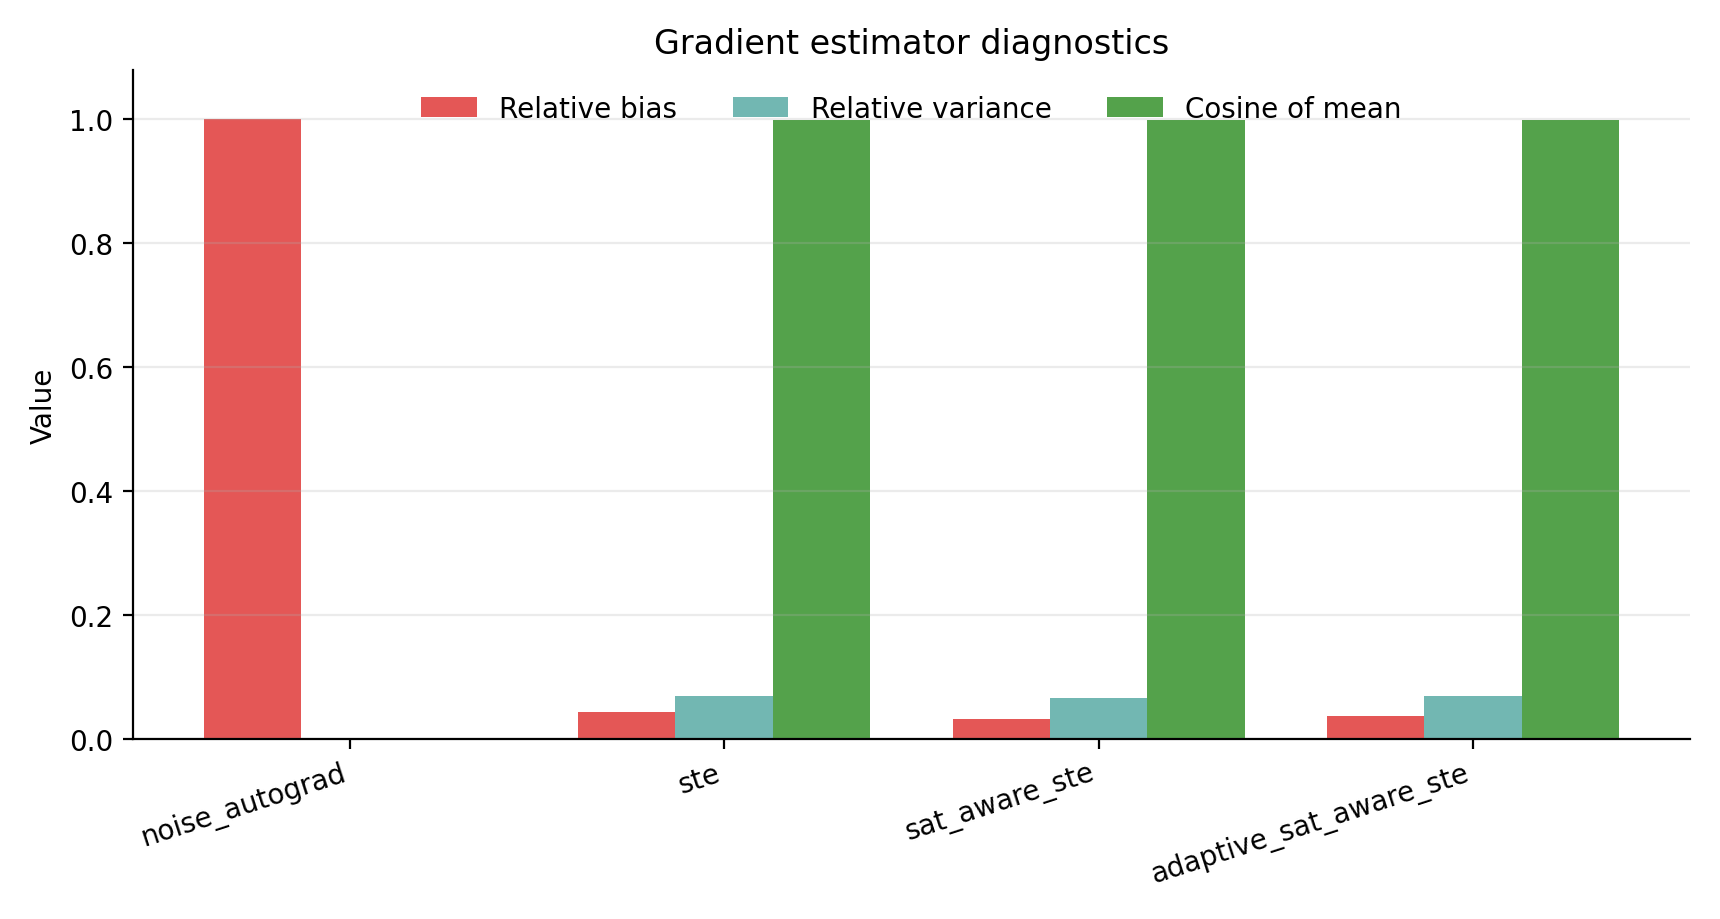
\includegraphics[width=\columnwidth]{gradient_diagnostics.png}
  \caption{Gradient diagnostic comparing native noisy autograd, identity STE,
  and saturation-aware estimators.  Native differentiation has a zero weight
  gradient through the quantized path in this probe; saturation-aware STE has
  mean-gradient cosine 0.9995 and relative bias 0.0331.}
  \label{fig:gradient_diag}
\end{figure}

\begin{figure}[h]
  \centering
  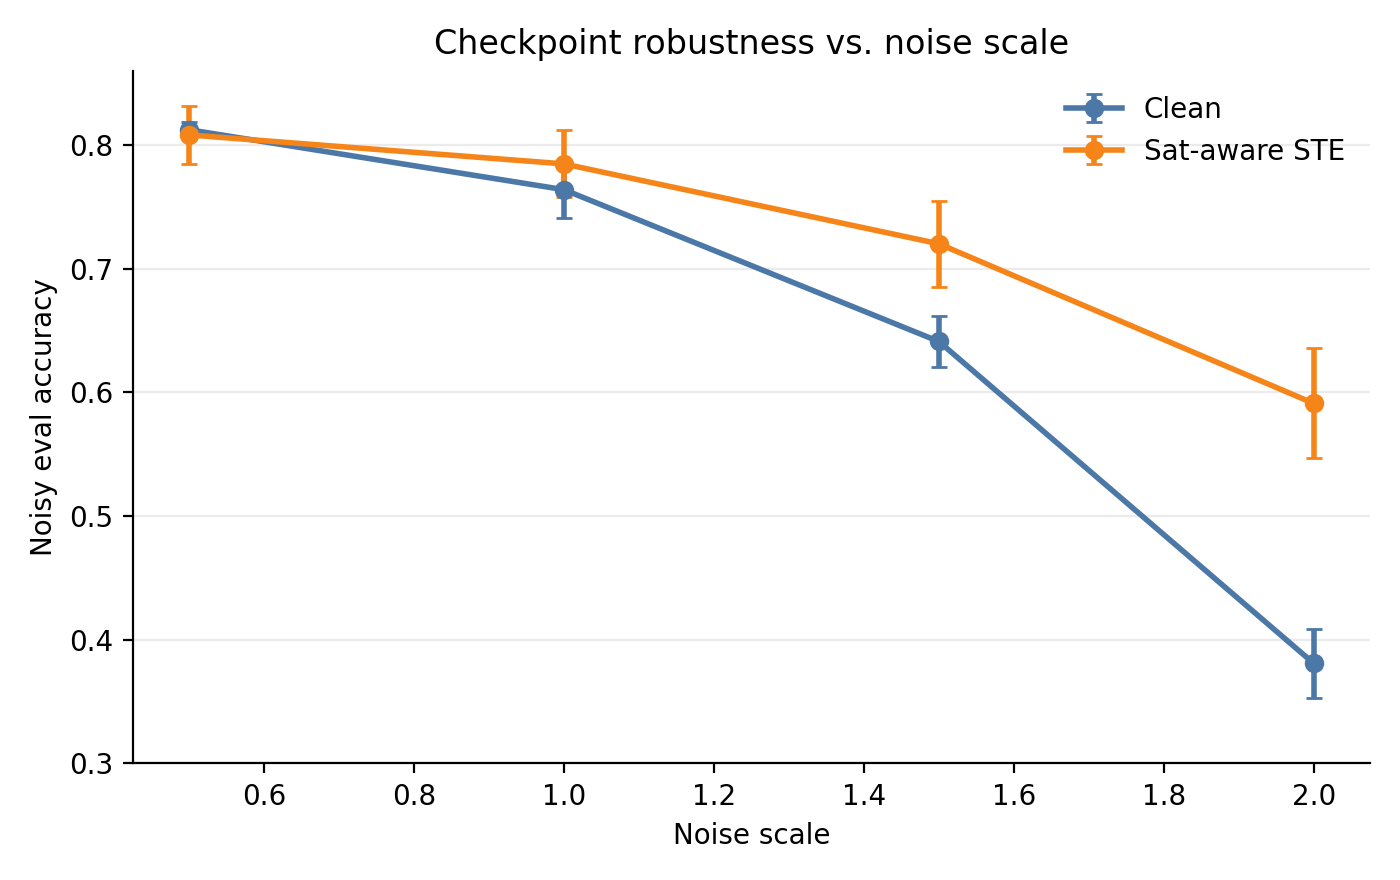
\includegraphics[width=\columnwidth]{noise_scale_sweep.png}
  \caption{Checkpoint robustness as the complete noise configuration is scaled.
  STE-trained checkpoints degrade more slowly than direct clean-to-noisy
  deployment at high noise.  This sweep is diagnostic; the main tables always
  use scale 1.0.}
  \label{fig:noise_sweep}
\end{figure}

Layer-wise calibrated TinyImageNet EfficientNet-B0 reaches
$80.09\%\mathbin{\pm}0.12\%$ by assigning lower noise coefficients to selected
pointwise and linear layers.  This value is useful as a hardware-mapping upper
bound, but it violates the strict uniform-noise protocol and is excluded from
all main rankings.  Similarly, bypassing depthwise layers is retained only as a
diagnostic that identifies topology sensitivity.

\section{Extended-Task Diagnostics and Scope}
\label{app:optional}

The reported large-image results use physical shared-read state: weight-side
programming, drift, retention, temperature, and supply draws are reused across
all implementation chunks belonging to one physical read.  Input crosstalk and
output noise remain location-specific.  This makes the result invariant to the
chosen memory-bounding chunk size.

Corrected subsystem diagnostics give residual-to-signal ratios of 0.523, 0.676,
0.825, and 1.096 for the detection backbone, FPN, RPN, and ROI modules.  The
segmentation backbone, classifier, and auxiliary classifier obtain 0.756,
1.077, and 0.913.  These finite, shape-consistent traces indicate a genuine
head-sensitivity problem rather than an execution failure.

Three-seed paired comparisons require a positive mean delta, all seeds positive,
and paired $p<0.05$ for statistical support.  Online segmentation satisfies
these criteria with $+0.245\pp$, but does not improve the best absolute
full-validation result after one epoch.  Online detection and proposal-aligned
ROI supervision retain at least one negative seed and are reported as
non-significant mechanism studies.

\section{Reproducibility}
\label{app:reproducibility}

The implementation uses PyTorch \citep{paszke2019pytorch}.  The repository
contains the environment specification, fixed experiment configurations,
dataset-free smoke test, 48 unit tests, table reconstruction, and artifact hash
verification.  From the repository root, the compact integrity check is:
\begin{verbatim}
conda env create -f environment.yml
conda activate imc-ste
python scripts/verify_project.py
\end{verbatim}
The verification command runs the clean/noisy/STE and online-profile smoke
paths, the test suite, arithmetic checks for reported results, and deterministic
regeneration of the key table and figure.  Public datasets and large
checkpoints are intentionally excluded from the compact submission archive;
the repository README records data preparation, full training, and checkpoint
evaluation commands.

\end{document}
